\documentclass[a4paper,14pt]{extarticle}

\usepackage[utf8x]{inputenc}
\usepackage[T1,T2A]{fontenc}
\usepackage[russian]{babel}
\usepackage{hyperref}
\usepackage{indentfirst}
\usepackage{here}
\usepackage{array}
\usepackage{graphicx}
\usepackage{caption}
\usepackage{subcaption}
\usepackage{chngcntr}
\usepackage{amsmath}
\usepackage{amssymb}
\usepackage{pgfplots}
\usepackage{pgfplotstable}
\usepackage[left=2cm,right=2cm,top=2cm,bottom=2cm,bindingoffset=0cm]{geometry}
\usepackage{multicol}

\renewcommand{\le}{\ensuremath{\leqslant}}
\renewcommand{\leq}{\ensuremath{\leqslant}}
\renewcommand{\ge}{\ensuremath{\geqslant}}
\renewcommand{\geq}{\ensuremath{\geqslant}}
\renewcommand{\epsilon}{\ensuremath{\varepsilon}}
\renewcommand{\phi}{\ensuremath{\varphi}}

\counterwithin{figure}{section}
\counterwithin{equation}{section}
\counterwithin{table}{section}
\newcommand{\sign}[1][5cm]{\makebox[#1]{\hrulefill}} % Поля подписи и даты
\graphicspath{{pics/}} % Путь до папки с картинками
\captionsetup{justification=centering,margin=1cm}
\def\arraystretch{1.3}

\begin{document}

\begin{titlepage}
\begin{center}
	\textbf{Санкт-Петербургский Политехнический Университет \\Петра Великого}\\[0.3cm]
	\small Институт компьютерных наук и технологий \\[0.3cm]
	\small Кафедра компьютерных систем и программных технологий\\[4cm]
	
	\textbf{ОТЧЕТ}\\ \textbf{о лабораторной работе}\\[0.5cm]
	\textbf{<<Исследование частотных характеристик пассивных RC-цепей>>}\\[0.1cm]
	\textbf{Электротехника и Электроника}\\[10.5cm]
\end{center}

\begin{flushright}
	\begin{minipage}{0.60\textwidth}
		\begin{flushleft}
			\small \textbf{Работу выполнили студенты}\\[3mm]
			\small группа 23501/4 \hspace*{17mm} Дьячков В.В.\\[3mm]
			\small группа 23501/4 \hspace*{17mm} Ламтев А.Ю.\\[5mm]
			
			\small \textbf{Преподаватель}\\[5mm]
		 	\small \sign[3.5cm] \hspace*{8mm} к.т.н., доц. Кочетков Ю.Д.\\[0.5cm]
		\end{flushleft}
	\end{minipage}
\end{flushright}

\vfill

\begin{center}
	\small Санкт-Петербург\\
	\small \the\year
\end{center}
\end{titlepage}

\section{Цель работы}

Ознакомиться с принципом действия параметрического стабилизатора напряжения. Настроить и исследовать его. Рассчитать силовые звенья.

\section{Чертеж схемы исследуемого устройства}

\begin{figure}[H]
\begin{center}
	\begin{subfigure}[b]{0.45\textwidth}
		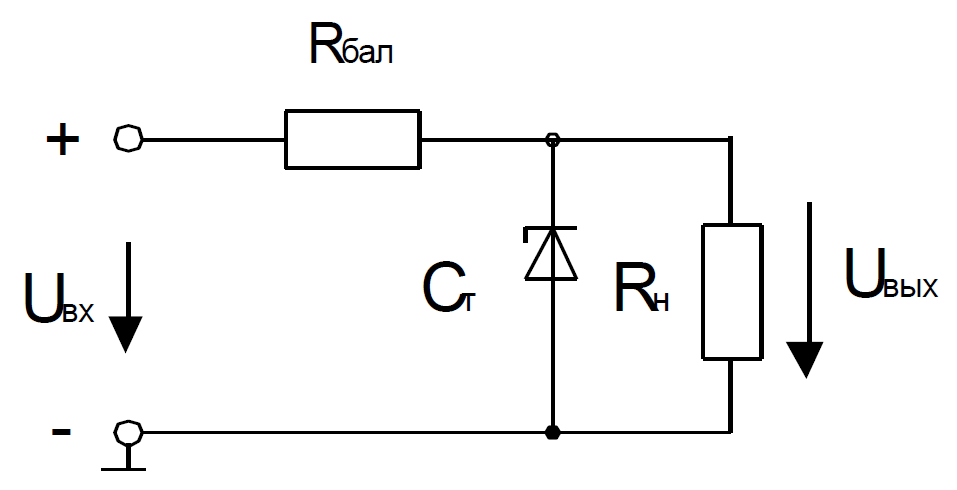
\includegraphics[scale=0.35]{stabilizer}
		\caption{Параметрический стабилизатор\\ постоянного напряжения}
	\end{subfigure}
	\begin{subfigure}[b]{0.45\textwidth}
		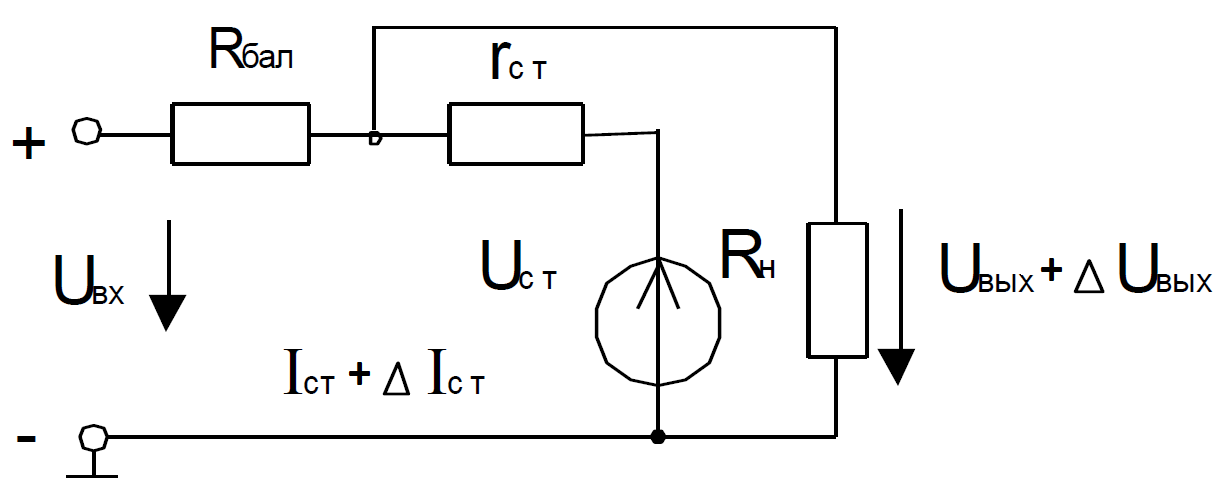
\includegraphics[scale=0.35]{substitution}
		\caption{Схема замещения \\стабилизатора}
	\end{subfigure}
	\caption{}
\end{center}
\end{figure}

\vspace{-0.5cm}

\section{Исходные данные}

\begin{table}[H]
\begin{center}
	\caption{Исходные данные}
	\def\tabcolsep{36pt}
	\begin{tabular}{|c|c|}
		\hline 
		$U_\text{вх}$ & 15 В \\ 
		\hline 
		$U_\text{вых}$ & 9 В \\ 
		\hline 
		$I_p$ & 8 мА \\ 
		\hline 
		$R_\text{н}$ & 500 Ом \\ 
		\hline 
	\end{tabular} 
\end{center}
\end{table}

\vspace{-0.5cm}

\begin{table}[H]
\begin{center}
	\caption{Характеристика стабилитрона \texttt{КС156А}}
	\def\tabcolsep{30pt}
	\begin{tabular}{|c|c|}
		\hline 
		$U$ & 5.6 В \\ 
		\hline 
		$I_{\text{ст}\ min}$ & 3 мА \\ 
		\hline 
		$I_{\text{ст}\ max}$ & 50 мА \\ 
		\hline 
		$r_{\text{ст}}$ & $\leq$ 46 Ом \\ 
		\hline 
	\end{tabular} 
\end{center}
\end{table}

\section{Теоретические расчеты и зависимости}

\subsection{Расчет параметров элементов и характеристик\\ стабилизатора}

\[
I_\text{вых} = \frac{U_\text{вых}}{R_\text{н}} = \frac{9}{500} = 0.018 \text{ A}
\]

\[
R_\text{бал} = \frac{U_\text{вх} - U_\text{вых}}{I_p + I_\text{вых}} = \frac{15 - 9}{0.008 + 0.018} = 230.769 \text{ Ом}
\]

\[
U_{\text{вх}\ min} = U_\text{вых} + R_\text{бал} \cdot (I_{\text{ст}\ min} + I_\text{вых}) = 9 + 230.769 \cdot (0.003 + 0.018) = 13.846 \text{ В}
\]
\[
U_{\text{вх}\ max} = U_\text{вых} + R_\text{бал} \cdot (I_{\text{ст}\ max} + I_\text{вых}) = 9 + 230.769 \cdot (0.05 + 0.018) = 24.692 \text{ В}
\]

\[
I_{\text{вых}\ min} = 0
\]
\[
I_{\text{вых}\ max} = \frac{U_\text{вх} - U_\text{вых} - I_{\text{ст}\ min} \cdot R_\text{бал}}{R_\text{бал}} = \frac{15 - 9 - 0.003 \cdot 230.769}{230.769} = 0.023 \text{ А}
\]

\[
R_{\text{н}\ min} = \frac{U_\text{вых}}{I_{\text{вых}\ max}} = \frac{9}{0.023} = 391 \text{ Ом}
\]
\[
R_{\text{н}\ max} = \frac{U_\text{вых}}{I_{\text{вых}\ min}} = \frac{9}{0} = \infty \text{ Ом}
\] 

\subsection{Расчет коэффициента стабилизации и выходного\\ сопротивления}

Коэффициент стабилизации можно определить теоретически, исходя из параметров схемы:

\begin{equation}\label{eq:k_st}
K_\text{ст} = \frac{R_\text{бал}}{r_\text{ст}}
\end{equation}
\[
K_\text{ст} = \frac{R_\text{бал} \cdot U_\text{вых}}{r_\text{ст} \cdot U_\text{вх}} \geq \frac{230.769}{46} = 5.02
\]

\vspace{0.5cm}

Выходное сопротивление прибризительно равно дифференциальному сопротивлению стабилизатора:

\begin{equation}\label{eq:r_out}
R_\text{вых} \approx r_{\text{ст}}
\end{equation}
\[
R_\text{вых} \approx r_{\text{ст}} \leq 46 \text{ Ом}
\]

\section{Экспериментально снятые зависимости}

\subsection{Зависимость $U_\text{вых}$ от $U_\text{вх}$}

В таблице \ref{tab:u_in} и на рисунке \ref{fig:u_in} приведена зависимость $U_\text{вых}$ от $U_\text{вх}$.

\begin{table}[H]
\begin{center}
	\caption{Зависимость $U_\text{вых}$ от $U_\text{вх}$}
	\label{tab:u_in}
	\def\tabcolsep{40pt}
	\pgfplotstabletypeset[col sep=comma,
	    columns={u_in,u_out},
	    column type/.add={|c|}{},
	    columns/u_in/.style={fixed, precision=2, zerofill, column name={$U_\text{вх}$, В}},
	    columns/u_out/.style={fixed, precision=2, zerofill, column name={$U_\text{вых}$, В}},
	    every nth row={1}{before row=\hline},
	    every head row/.style={before row=\hline, after row=\hline},
	    every last row/.style={after row=\hline}
	   ]{data/u_in.csv}
\end{center}
\end{table}

На основе полученных данных был расчитан коэффициент стабилизации:

\[
K_\text{ст} = \frac{\Delta U_\text{пит}}{\Delta U_\text{ст}} = \frac{24.60 - 9.04}{5.58 - 5.00} = 26.83
\]

\begin{figure}[H]
\begin{center}
	\begin{tikzpicture} [every plot/.append style={thick}]
		\begin{axis}[
			height=0.4\textheight,
			width=0.9\textwidth,
			xlabel={$U_\text{вх}$, В},
			ylabel={$U_\text{вых}$, В},
			xlabel near ticks,
			ylabel near ticks,
			xmin=0,
			xmax=28,
			ymin=0,
			ymax=6,
			xtick={0,4,...,28},
			grid=major
		]
		\addplot table[x=u_in,y=u_out,col sep=comma]{data/u_in.csv};
		\end{axis}
	\end{tikzpicture}
	\caption{Зависимость $U_\text{вых}$ от $U_\text{вх}$}
	\label{fig:u_in}
\end{center}
\end{figure}

\newpage

\subsection{Зависимость $U_\text{вых}$ от $R_\text{н}$}

В таблице \ref{tab:r_n} и на рисунке \ref{fig:r_n} приведена зависимость $U_\text{вых}$ от $R_\text{н}$. На рисунке \ref{fig:i_n} приведена зависимость $U_\text{вых}$ от $I_\text{н}$.

\begin{table}[H]
\begin{center}
	\caption{Зависимость $U_\text{вых}$ от $R_\text{н}$}
	\label{tab:r_n}
	\def\tabcolsep{35pt}
	\pgfplotstabletypeset[col sep=comma,
	    columns={r_n,u_out,i_n},
	    column type/.add={|c|}{},
	    columns/r_n/.style={fixed, precision=2, zerofill, column name={$R_\text{н}$, Ом}},
	    columns/u_out/.style={fixed, precision=2, zerofill, column name={$U_\text{вых}$, В}},
	    columns/i_n/.style={fixed, precision=2, zerofill, column name={$I_\text{н}$, мА}},
	    every nth row={1}{before row=\hline},
	    every head row/.style={before row=\hline, after row=\hline},
	    every last row/.style={after row=\hline}
	   ]{data/r_n.csv}
\end{center}
\end{table}

Рассчитано уточненное значение $r_\text{ст}$:

\[
r_\text{ст} = R_\text{вых} = \frac{\Delta U_\text{ст}}{\Delta I_\text{н}} = \frac{5.47 - 5.30}{\left| 2.82 - 21.36 \right| \cdot 10^{-3}} = 9.17 \text{ Ом}
\]

\begin{figure}[H]
\begin{center}
	\begin{tikzpicture} [every plot/.append style={thick}]
		\begin{axis}[
			height=0.4\textheight,
			width=0.9\textwidth,
			xlabel={$R_\text{н}$, Ом},
			ylabel={$U_\text{вых}$, В},
			xlabel near ticks,
			ylabel near ticks,
			xmin=0,
			xmax=2000,
			ymin=0,
			ymax=6,
			xtick={0,250,...,2000},
			grid=major
		]
		\addplot table[x=r_n,y=u_out,col sep=comma]{data/r_n.csv};
		\end{axis}
	\end{tikzpicture}
	\caption{Зависимость $U_\text{вых}$ от $R_\text{н}$}
	\label{fig:r_n}
\end{center}
\end{figure}

\vspace{-1cm}

\begin{figure}[H]
\begin{center}
	\begin{tikzpicture} [every plot/.append style={thick}]
		\begin{axis}[
			height=0.4\textheight,
			width=0.9\textwidth,
			xlabel={$I_\text{н}$, мА},
			ylabel={$U_\text{вых}$, В},
			xlabel near ticks,
			ylabel near ticks,
			xmin=0,
			xmax=60,
			ymin=0,
			ymax=6,
			xtick={0,10,...,60},
			grid=major
		]
		\addplot table[x=i_n,y=u_out,col sep=comma]{data/r_n.csv};
		\end{axis}
	\end{tikzpicture}
	\caption{Зависимость $U_\text{вых}$ от $I_\text{н}$}
	\label{fig:i_n}
\end{center}
\end{figure}

\section{Анализ экспериментальных вычислений}

Получив $r_\text{ст}$, вычислим уточненное теоретическое значение $K_\text{ст}$:

\[
K_\text{ст\ теор\ уточн} = \frac{R_\text{бал}}{r_\text{ст}} = \frac{230.77}{9.17} = 25.16
\]

\[
\delta K_\text{ст} = \frac{\left| K_\text{ст\ теор\ уточн} - K_\text{ст\ эксп} \right|}{K_\text{ст\ теор\ уточн}} = \frac{\left| 25.16 - 26.83 \right|}{25.16} = 0.066 = 6.6~\%
\]

\section{Выводы}

Значение $K_\text{ст}$, вычисленное в ходе эксперимента, близко к уточненному теоретическому значению ($\delta = 6.6~\%$). Таким образом, теоретические формулы \ref{eq:k_st} и \ref{eq:r_out}  являются верными.

\end{document}